\appendix
\chapter{Appendix for Chapter~\ref{chap:Tides}}
%%%%%%%%%%%%%%%%%%%%%%%%%%%%%%%%%%%%%%%%%%%%%%%%%%%
%%%%%%%%%%%%%%%%%%%%%%%%%%%%%%%%%%%%%%%%%%%%%%%%%%%
%%%%%%%%%%%%%%%%%%%%%%%%%%%%%%%%%%%%%%%%%%%%%%%%%%%
\section{Calculation of Minimum Eccentricity Required for Inner Planet Given $\Delta_{obs}$ and $T$ Years}
\label{app:min_e}

Starting from Eq.~\ref{eq:LiWu}, we now derive Eq.~\ref{eq:emin}:
\begin{equation*}
\frac{\dot{a}}{a} = 2e\dot{e}
\end{equation*}
\begin{equation}
\frac{da}{a} = 2e^2\frac{\dot{e}}{e}dt
\label{eq:daa}
\end{equation}
Since $\tau_e \equiv - \dot{e}/e$ is a constant, the only quantity with a time dependence on the right hand side is $e$.  
Integrating Eq.~\ref{eq:tidee} gives us an expression for $e(t)$:
\begin{equation*}
\frac{de}{e} = -\frac{9}{2}\pi \frac{k}{Q} \frac{1}{m_p} \sqrt{\frac{GM^3}{a^3}} \left(\frac{r_p}{a} \right)^5 dt =  \frac{\dot{e}}{e} dt  = -\frac{1}{\tau_e} dt
\end{equation*}
Since (again) we assume $\tau_e \equiv - e/\dot{e}$ is a constant, the integration is straightforward to yield:
\begin{equation}
e(t) = e_i \exp\left(-\frac{1}{\tau_e} t \right)
\label{eq:et}
\end{equation}

Now that we have eccentricity as a function of time, we can plug Eq.~\ref{eq:et} into Eq.~\ref{eq:daa} and integrate to get:
\begin{equation*}
\int_{a_i}^{a_f} \frac{da}{a} = 2e_i^2 \int_{0}^{T} \frac{-1}{\tau_e} \exp\left(-2\frac{1}{\tau_e} t \right) dt
\end{equation*}
\begin{equation}
\ln(a_i/a_f) = e_i^2 \left(1 - \exp(-2\frac{1}{\tau_e}T) \right)
\label{eq:X}
\end{equation}
We rearrange Eq.~\ref{eq:X} for $e_i$ to get:
\begin{equation}
e_i = \sqrt{\frac{\ln(a_i/a_f)}{1 - \exp(-2T/\tau_e)}}
\label{eq:ei}
\end{equation}
Where all quantities refer to a single planet (e.g. the inner planet). 
To connect Eq.~\ref{eq:ei} to a 2:1 MMR pair, we plug in Eq.~\ref{eq:DeltaInitial} along with the fact that $a_{in,i} = a_{out,i}/2^{2/3}$ (for 2:1 MMR) to get:
\begin{equation*}
e_{in,i} = \sqrt{\frac{\ln(a_i/a_f)_{in}}{1 - \exp(-2T/\tau_{e,in})}}
\end{equation*}
\begin{equation*}
e_{in,i} = \sqrt{\frac{\ln[(\frac{a_{out,i}}{2^{2/3}}) (\frac{(\Delta_{obs} + 2)^{2/3}}{a_{out,f}}) ]}{1 - \exp(-2T/\tau_{e,in})}}
\end{equation*}
\begin{equation}
e_{in,i} = \sqrt{\frac{\ln[(\frac{a_i}{a_f})_{out} (\frac{\Delta_{obs} + 2}{2})^{2/3}]}{1 - \exp(-2T/\tau_{e,in})}}
\end{equation}
Which is the result displayed in Eq.~\ref{eq:emin}.

%%%%%%%%%%%%%%%%%%%%%%%%%%%%%%%%%%%%%%%%%%%%%%%%%%%
%%%%%%%%%%%%%%%%%%%%%%%%%%%%%%%%%%%%%%%%%%%%%%%%%%%
%%%%%%%%%%%%%%%%%%%%%%%%%%%%%%%%%%%%%%%%%%%%%%%%%%%
\section{Maximum Eccentricity From Dynamical Simulations}
\label{app:emax}
In constructing the blue shaded region in Figure~\ref{fig:emin}, we have performed numerical simulations of stability for each Kepler system.
We simulate each Kepler system for 2 Myr, and assign the same initial eccentricity $e_i$ to each planet in the system. 
We do not migrate these planets into resonance, but since (in general) resonance can add a destabilizing effect \citep{Chambers, Funk2010, Pu2015}, these simulations can be used as conservative upper limits for the maximum eccentricity that a system can have and remain stable.  
The results are presented in Figure~\ref{fig:emax_dyn}, and error bars are derived from Poisson statistics. 

\begin{figure}
\centerline{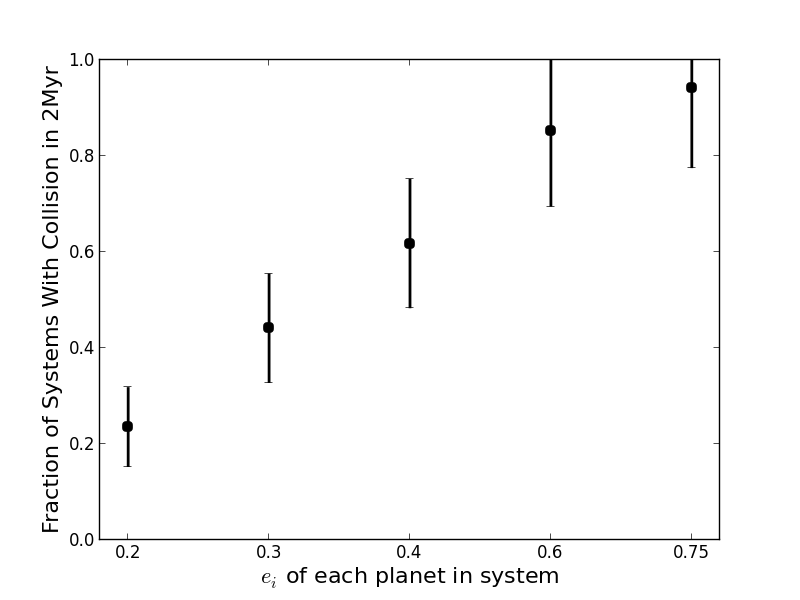
\includegraphics[trim=0cm 0cm 0.5cm 0.5cm, scale=0.48]{appendix/e_max_dyn.png}}
\caption{The fraction of \kep{} systems in our sample that go unstable within 2Myr if each planet is given an initial eccentricity of $e_i$. The error bars derived from Poisson statistics.}
\label{fig:emax_dyn}
\end{figure}

Each point in Figure~\ref{fig:emax_dyn} represents the fraction of systems in our sample having a collision within 2 Myr.
We can see that for $e_i = 0.3$, about half of the Kepler systems have had a collision. 
Thus from stability arguments, the maximum initial eccentricity that planets in our Kepler sample can have in order for $\sim 50\%$ of them to survive at least 2 Myr is $e_{max} \approx 0.3$.  

%%%%%%%%%%%%%%%%%%%%%%%%%%%%%%%%%%%%%%%%%%%%%%%%%%%
%%%%%%%%%%%%%%%%%%%%%%%%%%%%%%%%%%%%%%%%%%%%%%%%%%%
%%%%%%%%%%%%%%%%%%%%%%%%%%%%%%%%%%%%%%%%%%%%%%%%%%%
\onecolumn
\newpage
\section{Planet Sample}

\begin{center}
%\begin{longtable}{|c|c|c|c|p{2cm}|c|c|c|c|}
\begin{longtable}{rcrrrrrrr}
\caption[Portrait, single page table]{Kepler Systems Used In This Analysis} \\
 
\hline \hline \\[-0.1ex]
   \multicolumn{1}{c}{ {System}} &
   \multicolumn{1}{c}{ {Planet}} &
   \multicolumn{1}{c}{ {$P$ (days)}} &
   \multicolumn{1}{c}{ {near MMR}} &
   \multicolumn{1}{c}{ {$m_p/m_{\oplus}$}} &
   \multicolumn{1}{c}{ {$r_p/r_{\oplus}$}} &
   \multicolumn{1}{c}{ {$N_p$}}  &
   \multicolumn{1}{c}{ {$M/M_{\odot}$}} &
   \multicolumn{1}{c}{ {$R/R_{\odot}$}}  \\[0.5ex]\hline \hline \\[-2ex]
\endfirsthead

%\hline \kep{} System &  Planet Letter &  $P$ (days) & near MMR & $m_p/m_{\oplus}$ &  $r_p/r_{\oplus}$ & $N_p$ & $M/M_{\odot}$ &  $R/R_{\odot}$   \\\hline
KOI-142 & b & 10.95 & \checkmark & $8.7 \pm 2.5$ & $3.82 \pm 0.44$ & 2 & $0.96 \pm 0.04$ & $0.88 \pm 0.03$ \\  
 & c & 22.34 & \checkmark & $198.8 \pm 9.2$ & $6.82 \pm 1.09$ & & & \\  
\hline 
Kepler-120 & b & 6.31 & \checkmark & $  $ & $2.18 \pm 0.22$ & 2 & $  $ & $0.53 \pm 0.03$ \\  
 & c & 12.79 & \checkmark & $  $ & $1.53 \pm 0.11$ & & & \\  
\hline 
Kepler-127 & b & 14.44 & \checkmark & $  $ & $1.42 \pm 0.11$ & 3 & $  $ & $1.36 \pm 0.04$ \\  
 & c & 29.39 & \checkmark & $  $ & $2.62 \pm 0.11$ & & & \\  
 & d & 48.63 & & $  $ & $2.62 \pm 0.11$ & & & \\  
\hline 
Kepler-176 & b & 5.43 & & $  $ & $1.42 \pm 0.76$ & 3 & $  $ & $0.89 \pm 0.46$ \\  
 & c & 12.76 & \checkmark & $  $ & $2.62 \pm 1.31$ & & & \\  
 & d & 25.75 & \checkmark & $  $ & $2.51 \pm 1.31$ & & & \\  
\hline 
Kepler-183 & b & 5.69 & \checkmark & $  $ & $2.07 \pm 0.87$ & 2 & $  $ & $0.96 \pm 0.41$ \\  
 & c & 11.64 & \checkmark & $  $ & $2.29 \pm 0.98$ & & & \\  
\hline 
Kepler-221 & b & 2.8 & \checkmark & $  $ & $1.75 \pm 0.22$ & 4 & $0.72 \pm 0.05$ & $0.82 \pm 0.07$ \\  
 & c & 5.69 & \checkmark & $  $ & $2.95 \pm 0.33$ & & & \\  
 & d & 10.04 & & $  $ & $2.73 \pm 0.22$ & & & \\  
 & e & 18.37 & & $  $ & $2.62 \pm 0.22$ & & & \\  
\hline 
Kepler-244 & b & 4.31 & & $  $ & $2.73 \pm 1.2$ & 3 & $  $ & $0.8 \pm 0.34$ \\  
 & c & 9.77 & \checkmark & $  $ & $2.07 \pm 0.87$ & & & \\  
 & d & 20.05 & \checkmark & $  $ & $2.29 \pm 0.98$ & & & \\  
\hline 
Kepler-25 & b & 6.24 & \checkmark & $9.0 \pm 2.4$ & $2.62 \pm 0.0$ & 3 & $1.19 \pm 0.06$ & $1.31 \pm 0.02$ \\  
 & c & 12.72 & \checkmark & $14.3 \pm 2.7$ & $4.48 \pm 0.0$ & & & \\  
 & d & 123.0 && $89.9 \pm 13.7$ & $5.46 \pm 0.0$ & & & \\  
\hline 
Kepler-267 & b & 3.35 & \checkmark & $  $ & $1.97 \pm 0.11$ & 3 & $0.56 \pm 0.05$ & $0.56 \pm 0.02$ \\  
 & c & 6.88 & \checkmark & $  $ & $2.07 \pm 0.11$ & & & \\  
 & d & 28.46 & & $  $ & $2.29 \pm 0.11$ & & & \\  
\hline 
Kepler-27 & b & 15.33 & \checkmark & $41.8 \pm 5.0$ & $4.04 \pm 0.0$ & 2 & $0.65 \pm 0.16$ & $0.59 \pm 0.15$ \\  
 & c & 31.33 & \checkmark & $21.2 \pm 3.2$ & $4.91 \pm 0.0$ & & & \\  
\hline 
Kepler-272 & b & 2.97 & \checkmark & $  $ & $1.42 \pm 0.76$ & 3 & $0.79 \pm 0.05$ & $0.93 \pm 0.5$ \\  
 & c & 6.06 & \checkmark & $  $ & $1.75 \pm 0.98$ & & & \\  
 & d & 10.94 & & $  $ & $2.29 \pm 1.2$ & & & \\  
\hline 
Kepler-30 & b & 29.33 & \checkmark & $11.3 \pm 1.4$ & $3.93 \pm 0.22$ & 3 & $0.99 \pm 0.08$ & $0.95 \pm 0.12$ \\  
 & c & 60.32 & \checkmark & $640.0 \pm 50.0$ & $12.34 \pm 0.44$ & & & \\  
 & d & 143.34 & & $23.1 \pm 2.7$ & $8.84 \pm 0.55$ & & & \\  
\hline 
Kepler-305 & b & 5.49 & & $10.5 \pm 2.6$ & $3.6 \pm 0.87$ & 3 & $0.76 \pm 0.13$ & $0.79 \pm 0.05$ \\  
 & c & 8.29 & \checkmark & $6.0 \pm 2.4$ & $3.28 \pm 0.76$ & & & \\  
 & d & 16.74 & \checkmark & $  $ & $2.73 \pm 0.44$ & & & \\  
\hline 
Kepler-32 & f & 0.74 & & $  $ & $0.76 \pm 0.11$ & 5 & $0.54 \pm 0.02$ & $0.53 \pm 0.02$ \\  
 & e & 2.9 & \checkmark & $  $ & $1.53 \pm 0.11$ & & & \\  
 & b & 5.9 & \checkmark & $9.4 \pm 3.6$ & $2.18 \pm 0.22$ & & & \\  
 & c & 8.75 & & $7.7 \pm 5.0$ & $1.97 \pm 0.22$ & & & \\  
 & d & 22.78 & & $  $ & $2.73 \pm 0.11$ & & & \\  
\hline 
Kepler-326 & b & 2.25 & \checkmark & $  $ & $1.53 \pm 0.22$ & 3 & $0.98 \pm 0.05$ & $0.8 \pm 0.05$ \\  
 & c & 4.58 & \checkmark & $  $ & $1.42 \pm 0.11$ & & & \\  
 & d & 6.77 & & $  $ & $1.2 \pm 0.11$ & & & \\  
\hline 
Kepler-327 & b & 2.55 & \checkmark & $  $ & $1.09 \pm 0.11$ & 3 & $0.55 \pm 0.05$ & $0.49 \pm 0.02$ \\  
 & c & 5.21 & \checkmark & $  $ & $0.98 \pm 0.11$ & & & \\  
 & d & 13.97 & & $  $ & $1.75 \pm 0.11$ & & & \\  
\hline 
Kepler-328 & b & 34.92 & \checkmark & $28.5 \pm 12.9$ & $2.29 \pm 0.98$ & 2 & $1.15 \pm 0.22$ & $1.06 \pm 0.44$ \\  
 & c & 71.31 & \checkmark & $39.4 \pm 13.6$ & $5.46 \pm 2.29$ & & & \\  
\hline 
Kepler-384 & b & 22.6 & \checkmark & $  $ & $1.09 \pm 0.33$ & 2 & $0.76 \pm 0.05$ & $0.88 \pm 0.25$ \\  
 & c & 45.35 & \checkmark & $  $ & $1.09 \pm 0.33$ & & & \\  
\hline 
Kepler-386 & b & 12.31 & \checkmark & $  $ & $1.42 \pm 0.76$ & 2 & $0.74 \pm 0.05$ & $0.77 \pm 0.43$ \\  
 & c & 25.19 & \checkmark & $  $ & $1.64 \pm 0.87$ & & & \\  
\hline 
Kepler-396 & b & 42.99 & \checkmark & $75.5 \pm 11.8$ & $3.49 \pm 1.31$ & 2 & $0.85 \pm 0.13$ & $1.06 \pm 0.39$ \\  
 & c & 88.5 & \checkmark & $17.9 \pm 2.8$ & $5.35 \pm 1.97$ & & & \\  
\hline 
Kepler-48 & b & 4.78 & \checkmark & $14.3 \pm 4.3$ & $2.18 \pm 0.0$ & 3 & $0.88 \pm 0.06$ & $0.89 \pm 0.05$ \\  
 & c & 9.67 & \checkmark & $9.8 \pm 3.3$ & $3.17 \pm 0.0$ & & & \\  
 & d & 42.9 & & $7.93 \pm 4.6$ & $2.07 \pm 0.11$ & & & \\  
\hline 
Kepler-56 & b & 10.5 & \checkmark & $22.1 \pm 3.9$ & $6.55 \pm 0.33$ & 2 & $1.32 \pm 0.13$ & $4.23 \pm 0.15$ \\  
 & c & 21.4 & \checkmark & $181.0 \pm 21.0$ & $9.83 \pm 0.44$ & & & \\  
\hline 
Kepler-57 & b & 5.73 & \checkmark & $118.1 \pm 24.1$ & $2.18 \pm 0.0$ & 2 & $0.83 \pm 0.05$ & $0.73 \pm 0.0$ \\  
 & c & 11.61 & \checkmark & $7.4 \pm 9.4$ & $1.53 \pm 0.0$ & & & \\  
\hline 
Kepler-79 & b & 13.48 & \checkmark & $  $ & $2.62 \pm 0.76$ & 4 & $1.1 \pm 1.63$ & $1.4 \pm 0.25$ \\  
 & c & 27.4 & \checkmark & $  $ & $2.73 \pm 0.87$ & & & \\  
 & d & 52.09 & & $  $ & $7.64 \pm 1.42$ & & & \\  
 & e & 81.07 & & $  $ & $3.38 \pm 0.66$ & & & \\  
\hline 
Kepler-81 & b & 5.96 & \checkmark & $  $ & $2.4 \pm 0.44$ & 3 & $0.64 \pm 0.38$ & $0.59 \pm 0.03$ \\  
 & c & 12.04 & \checkmark & $  $ & $2.4 \pm 0.33$ & & & \\  
 & d & 20.84 & & $  $ & $1.2 \pm 0.33$ & & & \\  
\hline 
Kepler-83 & d & 5.17 & & $  $ & $1.97 \pm 0.11$ & 3 & $0.66 \pm 0.41$ & $0.59 \pm 0.03$ \\  
 & b & 9.77 & \checkmark & $  $ & $2.84 \pm 0.44$ & & & \\  
 & c & 20.09 & \checkmark & $  $ & $2.4 \pm 0.33$ & & & \\  
\hline 
Kepler-9 & d & 1.59 & & $  $ & $1.64 \pm 0.22$ & 3 & $1.07 \pm 0.05$ & $1.02 \pm 0.05$ \\  
 & b & 19.24 & \checkmark & $80.09 \pm 4.13$ & $9.5 \pm 0.76$ & & & \\  
 & c & 38.91 & \checkmark & $54.35 \pm 4.13$ & $9.28 \pm 0.76$ & & & \\ 
\hline 

\label{tab:kepsys}
\end{longtable}
\end{center}
\twocolumn

\end{document}
